\documentclass[11pt,a4paper]{article}

\input{glyphtounicode}
\pdfgentounicode=1

\usepackage[utf8]{inputenc}
\usepackage[T1]{fontenc}
\usepackage{amsmath,amssymb,amsfonts,amsthm}
\usepackage{graphicx}
\usepackage{hyperref}
\usepackage{cite}
\usepackage{geometry}
\usepackage{booktabs}
\usepackage{microtype}
\usepackage{bm}

\newcommand{\bOmega}{\mathbf{\Omega}}
\newcommand{\bLambda}{\mathbf{\Lambda}}
\newcommand{\bPhi}{\mathbf{\Phi}}

\geometry{margin=1in}
\emergencystretch=1.5em

\hypersetup{
    colorlinks=true,
    linkcolor=blue,
    citecolor=red,
    urlcolor=cyan,
    pdftitle={Closed-Form Moment Reduction of 3D Space-Charge Fields for Fast Feedback in High-Intensity Hadron Rings},
    pdfauthor={Hyo Eun Ahn}
}

\newtheorem{theorem}{Theorem}
\newtheorem{lemma}[theorem]{Lemma}
\newtheorem{corollary}[theorem]{Corollary}

\title{\textbf{Closed-Form Moment Reduction of 3D Space-Charge Fields for Fast Feedback in High-Intensity Hadron Rings}}

\author{
    \textbf{Hyo Eun Ahn}\thanks{Email: ahn@aya.yale.edu} \\
    \textit{Independent Researcher}
}

\date{\today}

\begin{document}

\maketitle

\begin{abstract}
In high-intensity hadron accumulator rings, rapid-cycling synchrotrons, and low-to-medium energy injector boosters---such as the Los Alamos Proton Storage Ring (PSR), the Spallation Neutron Source (SNS) accumulator ring, the CERN Proton Synchrotron Booster (PSB), and FAIR SIS18---intense self-induced Coulomb repulsion inside dense particle bunches ($\gamma \sim 1.15\text{--}3.1$) drives large incoherent space-charge tune shifts ($\Delta Q_{\mathrm{sc}} \sim -0.1 \text{ to } -0.4$), resulting in envelope mismatch resonances, transverse emittance growth, and halo generation. While active damping of dipolar centroid oscillations has been standard practice since Simon van der Meer's stochastic cooling, real-time active compensation of higher-order space-charge fields remains computationally challenging due to the millisecond-to-second latency of direct $O(N^2)$ Coulomb summation and grid-based $O(N_p + G \log G)$ Particle-in-Cell (PIC) solvers relative to the sub-microsecond to microsecond revolution period ($T_{\mathrm{rev}} \approx 0.36\text{--}1.0\,\mu\mathrm{s}$, or $\le 5\,\mu\mathrm{s}$ for a 5-turn envelope control window). In this paper, building on the author's 1994 Los Alamos space-charge moment formulations, we establish a closed-form reduced-order moment framework that evaluates 3D interior space-charge potential and electric-field polynomial coefficients via $35 \times 35$ and $34 \times 35$ matrix-vector kernels ($\sim 1.6\text{--}5.8\,\mu\mathrm{s}$ compute latency on a single CPU core, $\sim 5.4\text{--}20\,\mu\mathrm{s}$ including Python-level Zero-Self-Force indexing, and $< 1.0\,\mu\mathrm{s}$ projected on FPGA hardware for $1,247$ multiply-accumulate operations). By expanding the bunch distribution into $M=35$ spatial moments (all 3D monomials up to 4th order) and regularizing the underdetermined $N$-point mesh inversion ($\operatorname{rank}(\bOmega) = 35$) with a normalized physical reference prior ($\sum_{i=1}^N \mu_i = 1, \mu_i > 0$), strict pointwise positivity ($\bm{a} \equiv \bm{\mu} > \bm{0}$) is guaranteed at the reference equilibrium and fringe negative-charge overshoot is suppressed by $3.04\times$ ($0.2669 \to 0.0876$) in our 3D anisotropic bunch benchmark compared to Channell's uniform prior. Using reference-prior linearization ($\bm{w} = \bm{\mu}$), we demonstrate the exact algebraic ``fall-out'' of the mesh dimension $N$, collapsing the prior-weighted polynomial projection of the Plummer-softened Coulomb kernel into precomputed $35 \times 35$ potential ($\bm{v} = \bm{K}\bm{s} + \bm{v}_0$) and $34 \times 35$ electric-field ($\bm{v}_E^{\mathrm{prior}} = \bm{K}_E\bm{s} + \bm{v}_{E,0}$) matrices. Furthermore, because the uncorrected prior-weighted operator guarantees $\langle \bm{E}_{\mathrm{approx}}\rangle_{\bm{\mu}} = \langle \bm{E}_{\mathrm{exact}}\rangle_{\bm{\mu}}$ rather than vanishing net force on a perturbed state $\bm{a} = \bm{\mu} + \delta\bm{a}$ (where $\bm{\mu}^T \bm{G}\delta\bm{a} \ne \bm{0}$), we introduce an exact $O(M_E)$ moment-space Zero-Self-Force (ZSF) dipolar offset projection that restores $\langle \bm{E}_{\mathrm{approx}}^{\mathrm{ZSF}}\rangle_{\bm{a}} = \bm{0}$ to machine precision ($4.02 \times 10^{-16}$) without accessing the $N$-point mesh. In an idealized zero-latency multi-turn 2D transverse Leapfrog tracking and de-confounded ten-mode ablation study driven by self-consistent $O(N_p^2)$ 3D pairwise Plummer-Coulomb forces from identical initial conditions, we separate the physical roles of centroid-frame alignment and ZSF dipolar projection: aligning the polynomial evaluation frame with the moving beam centroid suppresses off-axis multipole feed-down (reducing RMS emittance growth from $+40.65\%$ open-loop to $+17.29\%$ for 11-term multipole correctors, $+13.45\%$ for the 34-basis operator, and $+6.40\%$ with a 2nd-moment rate damper), while Corollary~4's ZSF projection eliminates both polynomial and applied net self-force ($\sim 10^{-16}$) and suppresses spurious center-of-mass trajectory distortion ($0.049\text{--}0.081 \to \sim 10^{-17}$) purely from the 35 moments without altering central internal moments.
\end{abstract}

\noindent\textbf{Keywords:} Space-Charge Field Reduction, High-Intensity Hadron Rings, Injector Boosters, Moment Approach, Reduced-Order Modeling, Fast Multipole Feedback.

---

\section{Introduction}
The ultimate beam brightness ($N_b / \epsilon_n$) delivered by high-power proton drivers and hadron collider injector chains is fundamentally limited by collective space-charge forces at low and intermediate energies~\cite{reiser2008theory,baartman1998space}. In the laboratory frame, the self-generated magnetic force of a relativistic bunch partially cancels the electrostatic repulsion by a factor of $1 - \beta^2 = \gamma^{-2}$, so that the incoherent Laslett space-charge betatron tune shift scales inversely with $\beta \gamma^2$:
\begin{equation}
    \Delta Q_{\mathrm{sc}} = - \frac{r_p N_b F_g}{2 \pi \epsilon_n \beta \gamma^2 B_f},
    \label{eq:tune_shift}
\end{equation}
where $r_p = q^2 / (4\pi \epsilon_0 m_p c^2)$ is the classical proton radius, $N_b$ is the bunch intensity, $\epsilon_n$ is the normalized transverse RMS emittance, $\beta$ and $\gamma$ are the relativistic Lorentz factors, $B_f$ is the bunching factor, and $F_g$ is the transverse form factor. Consequently, while space-charge tune depression is negligible ($\Delta Q_{\mathrm{sc}} \sim 10^{-8}\text{--}10^{-9}$) at multi-TeV collider top energies~\cite{fcc2019conceptual}, it constitutes the primary intensity bottleneck in low-to-medium energy accumulator rings and injector boosters ($\gamma \sim 1.15\text{--}3.1$). Specifically, in machines such as the Los Alamos Proton Storage Ring (PSR, $E_k = 800\,\mathrm{MeV}$, $\gamma = 1.853$, circumference $C = 90.2\,\mathrm{m}$, revolution period $T_{\mathrm{rev}} = 0.358\,\mu\mathrm{s}$), the Spallation Neutron Source (SNS) accumulator ring ($E_k = 1.0\,\mathrm{GeV}$, $\gamma = 2.066$, $C = 248.0\,\mathrm{m}$, $T_{\mathrm{rev}} = 0.945\,\mu\mathrm{s}$)~\cite{henderson2014spallation}, the CERN Proton Synchrotron Booster (PSB, $E_k = 160\,\mathrm{MeV}\text{--}2.0\,\mathrm{GeV}$, $T_{\mathrm{rev}} = 0.57\text{--}1.01\,\mu\mathrm{s}$)~\cite{benedetto2015space}, and the FAIR SIS18 synchrotron~\cite{fair2006accelerator}, the incoherent tune depression reaches $|\Delta Q_{\mathrm{sc}}| \approx 0.1\text{--}0.4$.

When this large tune shift couples with injection envelope mismatch or pushes particles across low-order structure resonances ($m_x Q_x + m_y Q_y = k$), parametric collective resonances drive particles out of the high-density bunch core into an extended high-action halo~\cite{fedotov2003space}, causing beam loss and radioactivation of the ring aperture.

Historically, active feedback in circular accelerators has been restricted to dipolar (center-of-mass) centroid damping. Simon van der Meer's stochastic cooling~\cite{vandermeer1972stochastic,vandermeer1985nobel}, awarded the 1984 Nobel Prize in Physics, damps incoherent phase-space fluctuations over $10^4\text{--}10^7$ turns. By contrast, coherent envelope oscillations and space-charge-induced mismatch in compact high-intensity rings evolve over a few revolution turns ($T_{\mathrm{rev}} \approx 0.36\text{--}1.0\,\mu\mathrm{s}$, corresponding to a $5$-turn control window of $\le 5\,\mu\mathrm{s}$). Conventional self-consistent space-charge solvers cannot execute within this microsecond compute budget: direct pairwise Coulomb summation over $N$ mesh or macro-particle nodes scales as $O(N^2)$ ($\sim 1.6\,\mathrm{ms}$ even for $N=10^3$), while grid-based Fast Fourier Transform (FFT) or multigrid Particle-in-Cell (PIC) codes~\cite{birdsall2018plasma,qiang2000three} scale as $O(N_p + G \log G)$ for $N_p$ macro-particles and $G$ grid cells, requiring milliseconds to seconds per step.

In this work, we present the mathematical formalization and open-source numerical verification of a closed-form reduced-order Moment Approach to 3D space-charge field estimation and fast feedback control. It is important to distinguish the two components of this contribution:
\begin{enumerate}
    \item \textbf{1994 LANL Reduced-Order Moment Formulation (Sections~2--4.1)}: Originally motivated by Channell's moment dynamics~\cite{channell1993moment} and initiated during 1994 Los Alamos National Laboratory (LANL) studies for the BEDLAM code~\cite{ahn1994preliminary}, the author derived the normalized-prior affine charge inversion (`report1.pdf`), the weighted polynomial potential reduction (`poly-phi.pdf`), and the direct 3D vector electric-field reduction (`poly-e.pdf`), showing that the mesh dimension $N$ is algebraically eliminated offline into fixed $35 \times 35$ and $34 \times 35$ matrices.
    \item \textbf{2026 Moment-Space Zero-Self-Force (ZSF) Dipolar Offset Projection and De-Confounded Closed-Loop Feasibility Study (Sections~4.2--5)}: Extending the 1994 operator to modern real-time feedback, we resolve the non-zero self-force residual that arises when applying a fixed prior-weighted operator ($\bm{w}=\bm{\mu}$) to a perturbed beam distribution ($\bm{a} \ne \bm{\mu}$) via an exact $O(M_E)$ moment-space dipolar offset projection, and evaluate both coordinate-frame alignment and ZSF projection independently in a reproducible multi-turn 2D-in-3D pairwise-Coulomb Leapfrog tracking and ten-mode ablation benchmark.
\end{enumerate}

---

\section{Underdetermined Charge Inversion and Prior Regularization}

\subsection{Moment Representation in 3D Real Space}
In the co-moving rest frame of the bunch, let the spatial domain $\mathcal{V} \subset \mathbb{R}^3$ be discretized into $N$ mesh points $\bm{r}_i = (x_i, y_i, z_i)$ ($i = 1, \dots, N$). Let $a_i$ denote the normalized point-charge weight at mesh node $\bm{r}_i$, with $\bm{a} = [a_1, \dots, a_N]^T \in \mathbb{R}^N$.

The macroscopic geometry of the bunch is characterized by $M$ spatial moments up to polynomial order $P=4$:
\begin{equation}
    s_k = \langle m_k(\bm{r}) \rangle_{\bm{a}} = \sum_{i=1}^N m_k(\bm{r}_i) a_i, \quad k = 1, \dots, M,
    \label{eq:moments_def}
\end{equation}
where $m_k(\bm{r}) = x^{p_k} y^{q_k} z^{l_k}$ ($p_k + q_k + l_k \le 4$) are the $M = \binom{4+3}{3} = 35$ distinct 3D monomial basis functions:
\begin{equation}
    \bm{m}(\bm{r}) = \left[ 1, x, y, z, x^2, xy, xz, y^2, yz, z^2, x^3, \dots, z^4 \right]^T.
\end{equation}
Defining the moment evaluation matrix $\bOmega \in \mathbb{R}^{M \times N}$ with entries $\Omega_{ki} = m_k(\bm{r}_i)$, Eq.~\eqref{eq:moments_def} takes the linear form:
\begin{equation}
    \bm{s} = \bOmega \bm{a}.
    \label{eq:matrix_moment}
\end{equation}
When $N \gg M$ (typically $N \sim 10^3\text{--}10^5$ while $M = 35$) and the mesh points are non-coplanar on algebraic surfaces of degree $\le 4$ such that $\operatorname{rank}(\bOmega) = M = 35$, Eq.~\eqref{eq:matrix_moment} is an underdetermined linear inverse problem with an $(N - M)$-dimensional nullspace.

\subsection{Constrained Variational Inversion and Fringe Negativity Suppression}
To select a unique, smooth mesh charge assignment $\bm{a}$ without iterative non-negative quadratic programming (which would violate microsecond real-time constraints), we minimize the constrained quadratic functional~\cite{ahn1994preliminary}:
\begin{equation}
    \mathcal{J}(\bm{a}, \bm{\lambda}) = \frac{1}{2} \sum_{i=1}^N (a_i - \mu_i)^2 + \bm{\lambda}^T (\bm{s} - \bOmega \bm{a}),
    \label{eq:lagrangian_func}
\end{equation}
where $\bm{\mu} = [\mu_1, \dots, \mu_N]^T \in \mathbb{R}^N$ is a fixed reference prior distribution and $\bm{\lambda} \in \mathbb{R}^M$ is the Lagrange multiplier vector.

In early tests for the BEDLAM code at LANL, setting $\bm{\mu} = \bm{0}$ yielded the minimum-$L_2$-norm pseudoinverse solution $\bm{a}_{\min} = \bOmega^T (\bOmega\bOmega^T)^{-1} \bm{s}$, which exhibits large unphysical negative charge oscillations ($a_i < 0$) in the low-density bunch fringe whenever the bunch radius is smaller than the mesh radius ($R_{\mathrm{beam}} < R_{\mathrm{mesh}}$). Paul Channell suggested a uniform reference prior $\mu_i = \mathrm{const}$~\cite{channell1993moment}. However, because the zeroth-order constant monomial $m_1(\bm{r}) = 1$ lies in the row space of $\bOmega$, the orthogonal projection operator $[\bm{I}_N - \bOmega^T(\bOmega\bOmega^T)^{-1}\bOmega]$ annihilates any constant vector identically ($\|\bm{a}(\mu=\mathrm{const}) - \bm{a}(\mu=0)\|_\infty = 0$), leaving the fringe negativity unchanged.

As shown by the author in the April 1994 LANL study~\cite{ahn1994preliminary}, effective non-iterative regularization requires choosing a spatially localized physical reference profile $\bm{\mu}$ whose second moments match the nominal beam envelope and whose total weight is normalized to unity:
\begin{equation}
    \sum_{i=1}^N \mu_i = 1, \quad \mu_i > 0 \quad \forall i.
    \label{eq:mu_norm}
\end{equation}

\begin{theorem}[Closed-Form Affine Charge Reconstruction]
\label{thm:charge_inversion}
Assume the $N$-point 3D mesh satisfies the full-row-rank condition $\operatorname{rank}(\bOmega) = M = 35$, so that $\bOmega\bOmega^T \in \mathbb{R}^{35 \times 35}$ is strictly symmetric positive-definite. Under the normalization constraint~\eqref{eq:mu_norm}, the unique global minimizer of $\mathcal{J}(\bm{a}, \bm{\lambda})$ subject to $\bOmega\bm{a} = \bm{s}$ is the affine transformation:
\begin{equation}
    \bm{a} = \bm{\mu} + \bLambda (\bm{s} - \bOmega \bm{\mu}) = \bLambda \bm{s} + \bm{c},
    \label{eq:closed_a}
\end{equation}
where $\bLambda \in \mathbb{R}^{N \times M}$ is the Moore-Penrose right pseudoinverse and $\bm{c} \in \mathbb{R}^N$ is the prior residual vector:
\begin{equation}
    \bLambda = \bOmega^T (\bOmega \bOmega^T)^{-1}, \qquad \bm{c} = (\bm{I}_N - \bLambda \bOmega)\bm{\mu}.
    \label{eq:lambda_matrix}
\end{equation}
At the reference equilibrium ($\bm{s} = \bOmega \bm{\mu}$), Eq.~\eqref{eq:closed_a} yields $\bm{a} \equiv \bm{\mu} > \bm{0}$, guaranteeing strict pointwise positivity across all $N$ mesh points. For perturbed beams ($\bm{s} \ne \bOmega\bm{\mu}$), Eq.~\eqref{eq:closed_a} preserves all $M=35$ moments ($\bOmega\bm{a} = \bm{s}$) identically, and maintains pointwise positivity ($a_i > 0$) if and only if the moment perturbation satisfies the componentwise bound $[\bLambda(\bm{s} - \bOmega\bm{\mu})]_i > -\mu_i$.
\end{theorem}

\begin{proof}
Setting $\nabla_{\bm{a}} \mathcal{J} = \bm{0}$ gives $\bm{a} - \bm{\mu} - \bOmega^T \bm{\lambda} = \bm{0}$, or $\bm{a} = \bm{\mu} + \bOmega^T \bm{\lambda}$. Multiplying from the left by $\bOmega$ and enforcing $\bOmega\bm{a} = \bm{s}$ yields $\bOmega\bm{\mu} + (\bOmega\bOmega^T)\bm{\lambda} = \bm{s}$. Because $\operatorname{rank}(\bOmega) = M$, $\bOmega\bOmega^T$ is invertible, giving $\bm{\lambda} = (\bOmega\bOmega^T)^{-1}(\bm{s} - \bOmega\bm{\mu})$. Substituting $\bm{\lambda}$ back into $\bm{a}$ establishes Eq.~\eqref{eq:closed_a}, and the positivity condition $a_i > 0 \iff [\bLambda(\bm{s} - \bOmega\bm{\mu})]_i > -\mu_i$ follows immediately.
\end{proof}

\noindent\textbf{Remark on Finite Perturbations Outside the Positivity Neighborhood:}
Outside the perturbative neighborhood $[\bLambda(\bm{s} - \bOmega\bm{\mu})]_i > -\mu_i$, unconstrained affine inversion permits localized negative weights ($a_i < 0$) in the low-density fringe when $R_{\mathrm{beam}} < R_{\mathrm{mesh}}$. However, because $\bm{c} = (\bm{I}_N - \bLambda\bOmega)\bm{\mu}$ supplies the positive nullspace component of the localized reference profile $\bm{\mu}$, empirical evaluation on our 3D anisotropic bunch benchmark (Section~\ref{sec:verification_theorems}) demonstrates that Eq.~\eqref{eq:closed_a} reduces integrated fringe negative-charge overshoot by $3.04\times$ ($0.2669 \to 0.0876$) and $L_2$ reconstruction error by $2.00\times$ relative to the uniform/zero prior.

---

\section{Space-Charge Potential Reduction and the Fall-Out of \texorpdfstring{$N$}{N}}

\subsection{Interior Polynomial Potential Fitting via Weighted Least Squares}
Given a mesh charge distribution $\bm{a}$ in the bunch rest frame, the regularized discrete electrostatic potential on the mesh is given by the Plummer-softened Coulomb sum:
\begin{equation}
    \phi_{\mathrm{exact}}(\bm{r}_i) = \sum_{j=1}^N D_{ij} a_j, \qquad D_{ij} = \begin{cases} \dfrac{1}{\sqrt{|\bm{r}_i - \bm{r}_j|^2 + h^2}}, & i \ne j, \\[8pt] 0, & i = j, \end{cases}
    \label{eq:phi_exact}
\end{equation}
where $h = \alpha_h N^{-1/3}$ is the inter-particle mesh softening scale that prevents singular two-body collisions on the discrete grid and $D_{ii} = 0$ excludes self-interaction.

To represent the interior space-charge potential analytically within the beam core, we expand $\phi$ in the 4th-order monomial basis:
\begin{equation}
    \phi_{\mathrm{approx}}(\bm{r}) = \sum_{l=1}^M v_l m_l(\bm{r}) = \bm{m}^T(\bm{r}) \bm{v},
    \label{eq:phi_approx}
\end{equation}
where $\bm{v} = [v_1, \dots, v_M]^T \in \mathbb{R}^M$. Because a 4th-order polynomial grows as $r^4$ at large radii whereas the exterior Laplace potential decays as $r^{-1}$, an unweighted fit over the bounding box would be distorted by empty vacuum nodes outside the bunch. We therefore weight the least-squares functional by a positive density measure $w_i$ concentrated in the beam core:
\begin{equation}
    \chi^2_{\bm{w}}(\bm{v}) = \sum_{i=1}^N w_i \left[ \phi_{\mathrm{exact}}(\bm{r}_i) - \phi_{\mathrm{approx}}(\bm{r}_i) \right]^2.
    \label{eq:chi2_pot}
\end{equation}

\begin{theorem}[Potential Dimension Reduction and Weighted Moment Conservation]
\label{thm:potential_reduction}
For any weight vector $\bm{w} \in \mathbb{R}^N$ such that the weighted Gram matrix $\bOmega \{\bOmega\bm{w}\}^T \in \mathbb{R}^{M \times M}$ is non-singular (which holds whenever $w_i > 0$ on a rank-$M$ mesh), the normal equations minimizing $\chi^2_{\bm{w}}(\bm{v})$ yield the unique coefficient vector:
\begin{equation}
    \bm{v}(\bm{w}) = \bLambda^{\prime T}(\bm{w}) \bm{\phi}_{\mathrm{exact}}, \qquad \bLambda^{\prime}(\bm{w}) = \{\bOmega\bm{w}\}^T \Bigl[ \bOmega \{\bOmega\bm{w}\}^T \Bigr]^{-1},
    \label{eq:lambda_prime_def}
\end{equation}
where $\{\bOmega\bm{w}\}_{ki} = \Omega_{ki} w_i$. By virtue of the normal equations, the polynomial potential $\bm{\phi}_{\mathrm{approx}} = \bOmega^T \bm{v}(\bm{w})$ preserves all $M=35$ $\bm{w}$-weighted potential moments identically:
\begin{equation}
    \langle m_k \phi_{\mathrm{approx}} \rangle_{\bm{w}} = \sum_{i=1}^N w_i m_k(\bm{r}_i) \phi_{\mathrm{approx}}(\bm{r}_i) = \langle m_k \phi_{\mathrm{exact}} \rangle_{\bm{w}}, \qquad k = 1, \dots, M.
    \label{eq:pot_moment_conservation}
\end{equation}
Furthermore, adopting the fixed reference-prior weighting $\bm{w} = \bm{\mu}$ (first-order perturbative linearization around $\bm{a} = \bm{\mu}$) eliminates the mesh dimension $N$ entirely offline, yielding an algebraically exact reduced-order representation of the $\bm{\mu}$-weighted polynomial projection on the reconstructed charge $\bm{a} = \bLambda\bm{s} + \bm{c}$:
\begin{equation}
    \bm{v} = \bm{K} \bm{s} + \bm{v}_0, \qquad \bm{K} = \bLambda^{\prime T}(\bm{\mu}) \bm{D} \bLambda \in \mathbb{R}^{M \times M}, \qquad \bm{v}_0 = \bLambda^{\prime T}(\bm{\mu}) \bm{D} \bm{c} \in \mathbb{R}^M.
    \label{eq:matrix_magic}
\end{equation}
\end{theorem}

\begin{proof}
Setting $\partial \chi^2_{\bm{w}} / \partial v_k = 0$ for $k = 1, \dots, M$ yields the weighted normal equations:
\begin{equation}
    \sum_{i=1}^N w_i \Omega_{ki} \left( \bm{\Omega}^T \bm{v} \right)_i = \sum_{i=1}^N w_i \Omega_{ki} \phi_{\mathrm{exact}}(\bm{r}_i) \iff \{\bOmega\bm{w}\} \bOmega^T \bm{v} = \{\bOmega\bm{w}\} \bm{\phi}_{\mathrm{exact}},
    \label{eq:pot_normal}
\end{equation}
which establishes the moment conservation identity~\eqref{eq:pot_moment_conservation} and, upon left-multiplying by $[\{\bOmega\bm{w}\}\bOmega^T]^{-1}$, gives $\bm{v}(\bm{w}) = \bLambda^{\prime T}(\bm{w})\bm{\phi}_{\mathrm{exact}}$. Substituting $\bm{\phi}_{\mathrm{exact}} = \bm{D}\bm{a} = \bm{D}(\bLambda\bm{s} + \bm{c})$ with fixed weight $\bm{w} = \bm{\mu}$ factors all $N$-dimensional matrices into the offline constants $\bm{K}$ and $\bm{v}_0$ of Eq.~\eqref{eq:matrix_magic}.
\end{proof}

\noindent\textbf{Remark on Algebraic Reduction Exactness vs.\ Physical Field Approximation:}
It is essential to distinguish two levels of accuracy in Theorem~\ref{thm:potential_reduction}: (i) \emph{algebraic exactness of the reduced operator}, meaning that $\bm{v} = \bm{K}\bm{s} + \bm{v}_0 \in \mathbb{R}^{35}$ reproduces the full $N$-mesh prior-weighted projection $\bLambda^{\prime T}(\bm{\mu})\bm{D}(\bLambda\bm{s} + \bm{c})$ with zero truncation error ($1.14 \times 10^{-13}$ numerically), and (ii) \emph{physical field approximation}, which involves replacing the true continuum density by the affine reconstruction $\bm{a}$, truncating the potential basis at degree $P=4$, and replacing the state-dependent weight $\bm{w}=\bm{a}$ by the fixed prior weight $\bm{w}=\bm{\mu}$ (introducing an $O(\|\bm{a} - \bm{\mu}\|)$ difference relative to the state-weighted fit).

---

\section{Direct 3D Vector Electric Field Reduction and Moment-Space Zero-Self-Force Dipolar Offset Projection}

\subsection{Direct Vector Field Least-Squares Formulation}
In beam dynamics, betatron tune shifts and multipole kicks depend directly on the electric field $\bm{E} = -\nabla \phi$. Rather than differentiating a fitted scalar potential (which amplifies high-order boundary oscillations), the author derived a direct 3D vector electric-field least-squares fit in 1994 (`poly-e.pdf`).

Using the Plummer-softened field kernels $G_{x_j, ik} = (x_{j,i} - x_{j,k})(|\bm{r}_i - \bm{r}_k|^2 + h^2)^{-3/2}$ ($i \ne k$, $G_{x_j,ii} = 0$), the exact discrete electric field components along $x_1, x_2, x_3$ ($x, y, z$) are:
\begin{equation}
    \bm{E}_{x_j}^{\mathrm{exact}} = \bm{G}_{x_j} \bm{a}, \qquad j = 1, 2, 3.
    \label{eq:field_exact}
\end{equation}
Because the constant monomial $m_1(\bm{r}) = 1$ has zero gradient ($\nabla m_1 \equiv \bm{0}$), we retain only the $M_E = M - 1 = 34$ non-constant monomials ($1 \le p_l + q_l + l_l \le 4$), denoted by the reduced derivative matrices $\tilde{\bOmega}^{x_j} \in \mathbb{R}^{34 \times N}$ with entries $\tilde{\Omega}_{li}^{x_j} = \partial m_l(\bm{r}_i) / \partial x_j$. The polynomial electric field approximation is:
\begin{equation}
    \bm{E}_{x_j}^{\mathrm{approx}} = -\tilde{\bOmega}^{x_j T} \bm{v}_E, \qquad \bm{v}_E \in \mathbb{R}^{34}.
    \label{eq:field_approx}
\end{equation}
Minimizing the density-weighted 3D vector residual functional:
\begin{equation}
    \mathcal{S}_{\bm{w}}(\bm{v}_E) = \sum_{i=1}^N w_i \sum_{j=1}^3 \left[ E_{x_j}^{\mathrm{exact}}(\bm{r}_i) - E_{x_j}^{\mathrm{approx}}(\bm{r}_i) \right]^2,
    \label{eq:field_lsq}
\end{equation}
with respect to $\bm{v}_E$ yields the following theorem.

\begin{theorem}[Direct 3D Electric Field Reduction and Weighted Force Identity]
\label{thm:field_reduction}
For any weight vector $\bm{w} \in \mathbb{R}^N$ such that $\sum_{j=1}^3 \{\tilde{\bOmega}^{x_j} \bm{w}\} \tilde{\bOmega}^{x_j T} \in \mathbb{R}^{34 \times 34}$ is invertible, the optimal $34$-component electric-field coefficient vector minimizing $\mathcal{S}_{\bm{w}}(\bm{v}_E)$ is:
\begin{equation}
    \bm{v}_E(\bm{w}) = - \left[ \sum_{j=1}^3 \{\tilde{\bOmega}^{x_j} \bm{w}\} \tilde{\bOmega}^{x_j T} \right]^{-1} \left[ \sum_{j=1}^3 \{\tilde{\bOmega}^{x_j} \bm{w}\} \bm{E}_{x_j}^{\mathrm{exact}} \right].
    \label{eq:field_v_sol}
\end{equation}
This solution satisfies all $M_E = 34$ $\bm{w}$-weighted generalized field-moment normal equations identically:
\begin{equation}
    \sum_{j=1}^3 \left\langle \frac{\partial m_k}{\partial x_j} E_{x_j}^{\mathrm{approx}}(\bm{w}) \right\rangle_{\bm{w}} = \sum_{j=1}^3 \left\langle \frac{\partial m_k}{\partial x_j} E_{x_j}^{\mathrm{exact}} \right\rangle_{\bm{w}}, \qquad k = 2, \dots, 35.
    \label{eq:field_34_averages}
\end{equation}
In particular, evaluating Eq.~\eqref{eq:field_34_averages} for the three linear dipolar monomials $m_k \in \{x, y, z\}$ (where $\partial x_i / \partial x_j = \delta_{ij}$) guarantees the $\bm{w}$-weighted \textbf{Average Force Identity}:
\begin{equation}
    \langle \bm{E}_{\mathrm{approx}}(\bm{w}) \rangle_{\bm{w}} = \langle \bm{E}_{\mathrm{exact}} \rangle_{\bm{w}}.
    \label{eq:avg_force_preservation}
\end{equation}
Consequently:
\begin{enumerate}
    \item \textbf{State-Weighted Fit ($\bm{w} = \bm{a}$)}: By the antisymmetry $G_{x_j, ik} = -G_{x_j, ki}$ (Newton's third law), $\langle E_{x_j}^{\mathrm{exact}} \rangle_{\bm{a}} = \bm{a}^T \bm{G}_{x_j} \bm{a} = 0$, so the state-weighted fit satisfies $\langle \bm{E}_{\mathrm{approx}}(\bm{a}) \rangle_{\bm{a}} = \bm{0}$ identically.
    \item \textbf{Prior-Weighted Offline Reduction ($\bm{w} = \bm{\mu}$)}: Fixing $\bm{w} = \bm{\mu}$ collapses Eq.~\eqref{eq:field_v_sol} offline into the runtime $34 \times 35$ affine operator:
    \begin{equation}
        \bm{v}_E^{\mathrm{prior}} = \bm{K}_E \bm{s} + \bm{v}_{E,0}, \qquad \bm{K}_E = \bLambda_E^T(\bm{\mu}) \bLambda \in \mathbb{R}^{34 \times 35}, \qquad \bm{v}_{E,0} = \bLambda_E^T(\bm{\mu}) \bm{c} \in \mathbb{R}^{34},
        \label{eq:runtime_field_op}
    \end{equation}
    where $\bLambda_E^T(\bm{\mu}) = -\left[\sum_{j=1}^3 \{\tilde{\bOmega}^{x_j}\bm{\mu}\}\tilde{\bOmega}^{x_j T}\right]^{-1} \left(\sum_{j=1}^3 \{\tilde{\bOmega}^{x_j}\bm{\mu}\}\bm{G}_{x_j}\right) \in \mathbb{R}^{34 \times N}$. For a perturbed state $\bm{a} = \bm{\mu} + \delta\bm{a}$, Eq.~\eqref{eq:runtime_field_op} preserves the $\bm{\mu}$-weighted field averages $\langle E_{x_j}^{\mathrm{approx}}(\bm{\mu})\rangle_{\bm{\mu}} = \langle E_{x_j}^{\mathrm{exact}}\rangle_{\bm{\mu}} = \bm{\mu}^T \bm{G}_{x_j}\delta\bm{a} \ne 0$, which generally leaves a non-zero residual net force $\langle \bm{E}_{\mathrm{approx}}(\bm{\mu})\rangle_{\bm{a}} \ne \bm{0}$ on the actual distribution $\bm{a}$.
\end{enumerate}
\end{theorem}

\subsection{Exact Moment-Space Zero-Self-Force (ZSF) Dipolar Offset Projection}
As highlighted in Theorem~\ref{thm:field_reduction}, because $\bm{w}=\bm{\mu}$ is fixed offline, the uncorrected prior-weighted operator $\bm{v}_E^{\mathrm{prior}}$ does not automatically vanish when averaged over a perturbed charge state $\bm{a} \ne \bm{\mu}$: both $\bm{\mu}^T \bm{G}_{x_j} \delta\bm{a} \ne 0$ and the weighting mismatch $(\bm{a} - \bm{\mu})^T \bm{E}_{x_j}^{\mathrm{approx}}(\bm{\mu}) \ne 0$ contribute a spurious dipolar self-force $\langle \bm{E}_{\mathrm{approx}}(\bm{\mu}) \rangle_{\bm{a}} \ne \bm{0}$.

Crucially, because the spatial derivative of every monomial of degree $\le 4$ is a monomial of degree $\le 3$ already contained in $\bm{m}(\bm{r})$, there exist exact constant differentiation matrices $\bm{D}_{x_j}^{\mathrm{mom}} \in \mathbb{R}^{34 \times 35}$ such that $\tilde{\bOmega}^{x_j} \equiv \bm{D}_{x_j}^{\mathrm{mom}} \bOmega$. Therefore, for any polynomial coefficient vector $\bm{v}_E \in \mathbb{R}^{34}$ and any charge state $\bm{a}$ with moments $\bm{s} = \bOmega\bm{a}$, the instantaneous state-weighted net self-force depends \emph{exclusively on the $35$-element moment vector $\bm{s}$}:
\begin{equation}
    \langle E_{x_j}^{\mathrm{approx}} \rangle_{\bm{a}} = \bm{a}^T \left( -\tilde{\bOmega}^{x_j T} \bm{v}_E \right) = -\left( \bm{D}_{x_j}^{\mathrm{mom}} \bOmega \bm{a} \right)^T \bm{v}_E = -\left( \bm{D}_{x_j}^{\mathrm{mom}} \bm{s} \right)^T \bm{v}_E.
    \label{eq:moment_space_selfforce}
\end{equation}

\begin{corollary}[Moment-Space Zero-Self-Force (ZSF) Dipolar Offset Projection]
\label{cor:zsf_gauge}
Let $\bm{v}_E^{\mathrm{prior}} = \bm{K}_E\bm{s} + \bm{v}_{E,0} \in \mathbb{R}^{34}$ be the prior-weighted field coefficients, and let $l_x, l_y, l_z \in \{1,\dots,34\}$ denote the indices of the three linear dipolar basis monomials $(x, y, z)$, for which $(\bm{D}_{x_j}^{\mathrm{mom}}\bm{s})_{l_{x_k}} = \delta_{jk} s_{000}$. Defining the ZSF-projected coefficient vector $\bm{v}_E^{\mathrm{ZSF}} \in \mathbb{R}^{34}$ by leaving all $31$ higher-order multipole coefficients ($p+q+l \ge 2$) unchanged and setting the three spatially uniform dipolar components to:
\begin{equation}
    v_{E, l_{x_j}}^{\mathrm{ZSF}} = -\frac{1}{s_{000}} \sum_{\substack{l=1 \\ l \ne l_{x_j}}}^{34} v_{E, l}^{\mathrm{prior}} \left( \bm{D}_{x_j}^{\mathrm{mom}} \bm{s} \right)_l, \qquad j = 1, 2, 3,
    \label{eq:zsf_projection}
\end{equation}
enforces exact zero net self-force on the instantaneous perturbed distribution $\bm{a}$:
\begin{equation}
    \langle \bm{E}_{\mathrm{approx}}^{\mathrm{ZSF}} \rangle_{\bm{a}} = \langle \bm{E}_{\mathrm{exact}} \rangle_{\bm{a}} = \bm{0},
    \label{eq:zsf_exact_zero}
\end{equation}
in $O(M_E)$ scalar operations ($57$ non-zero derivative terms across $x, y, z$) using only $\bm{s} \in \mathbb{R}^{35}$, without accessing the $N$-point mesh or altering any quadrupolar, sextupolar, or octupolar field gradient. (We refer to Eq.~\eqref{eq:zsf_projection} as a \emph{dipolar offset projection} or \emph{zero-mean-force projection}, since adding a linear term $\delta\bm{c}\cdot\bm{r}$ to $\Phi_{\mathrm{poly}}$ shifts the spatially uniform dipolar field component $-\delta\bm{c}$ to satisfy Newton's third law, rather than shifting a constant scalar potential gauge.)
\end{corollary}

---

\section{Hardware Architecture and Numerical Verification}

\subsection{Moment Acquisition, Actuator Realizability, and Latency Budget}
In a physical synchrotron or accumulator ring, applying Eq.~\eqref{eq:runtime_field_op} and Corollary~\ref{cor:zsf_gauge} within a closed-loop feedback architecture involves three practical system constraints:
\begin{enumerate}
    \item \textbf{Hybrid Diagnostic-Observer Pipeline}: Standard wall-current monitors and 4-button/stripline Beam Position Monitors (BPMs) directly measure bunch intensity $s_{000}$, centroid offsets $(\langle x \rangle, \langle y \rangle, \langle z \rangle)$, and the transverse quadrupolar difference moment $\langle x^2 - y^2 \rangle$ (plus the skew-quadrupolar moment $\langle xy \rangle$ when equipped with rotated or 8-electrode pickups), whereas the quadrupolar sum $\langle x^2 + y^2 \rangle$ and 3rd- and 4th-order moments ($3 \le p+q+l \le 4$) are not directly observable from a single standard button BPM and require a synchronized online envelope/moment observer constrained by multi-BPM phase-advance tomography or periodic profile measurements.
    \item \textbf{Magnetic Corrector Realizability ($\bm{c}_{\mathrm{achievable}} = \bm{B}\bm{u}$)}: The $M_E = 34$ polynomial coefficients $\bm{v}_E^{\mathrm{ZSF}}$ parameterize an interior 3D electrostatic field ($\nabla\cdot\bm{E} \ne 0$ inside the bunch charge), whereas external magnetic correctors apply localized 2D transverse harmonic kicks satisfying Maxwell's vacuum equations ($\nabla\cdot\bm{B}_{\mathrm{ext}} = 0, \nabla\times\bm{B}_{\mathrm{ext}} = \bm{0}$). Thus, a physical corrector family with control currents $\bm{u}$ spans an achievable subspace $\bm{c}_{\mathrm{achievable}} = \bm{B}\bm{u}$. In our ablation study below, we explicitly contrast \textbf{Modes~B-Lab, B-CF, and B-CF-ZSF}---which restrict actuation to the $11$ low-order dipole, quadrupole, and octupole terms corresponding to standard corrector magnet families---against \textbf{Modes~C-Lab, C-CF, and C-CF-ZSF}, which apply all $34$ polynomial basis terms as a theoretical upper bound on 4th-order moment compensation.
    \item \textbf{Compute Kernel Latency vs.\ Total Closed-Loop Latency}: Total hardware loop delay is the sum of diagnostic acquisition, observer estimation, matrix computation, communication, and magnet power-supply/vacuum-chamber eddy-current response:
    \begin{equation}
        T_{\mathrm{total}} = T_{\mathrm{diag}} + T_{\mathrm{obs}} + T_{\mathrm{compute}} + T_{\mathrm{comm}} + T_{\mathrm{act}}.
        \label{eq:latency_budget}
    \end{equation}
    On a single CPU core, the $35 \times 35$ and $34 \times 35$ matrix-vector kernels execute in $\sim 1.6\text{--}5.8\,\mu\mathrm{s}$ in NumPy/OpenBLAS, while adding Python-level ZSF array indexing requires $\sim 5.4\text{--}20\,\mu\mathrm{s}$ (which slightly exceeds the $4.73\,\mu\mathrm{s}$ 5-turn window of the SNS ring in interpreted Python). Because the entire runtime operator consists of $34 \times 35 = 1,190$ matrix-vector multiply-accumulate (MAC) operations plus $57$ sparse ZSF derivative MACs ($1,247$ MACs total), compiled C or pipelined FPGA hardware executes $T_{\mathrm{compute}}$ in $< 1.0\,\mu\mathrm{s}$, demonstrating that the reduced-order space-charge field solver is no longer the computational bottleneck.
\end{enumerate}

\begin{figure}[htbp]
    \centering
    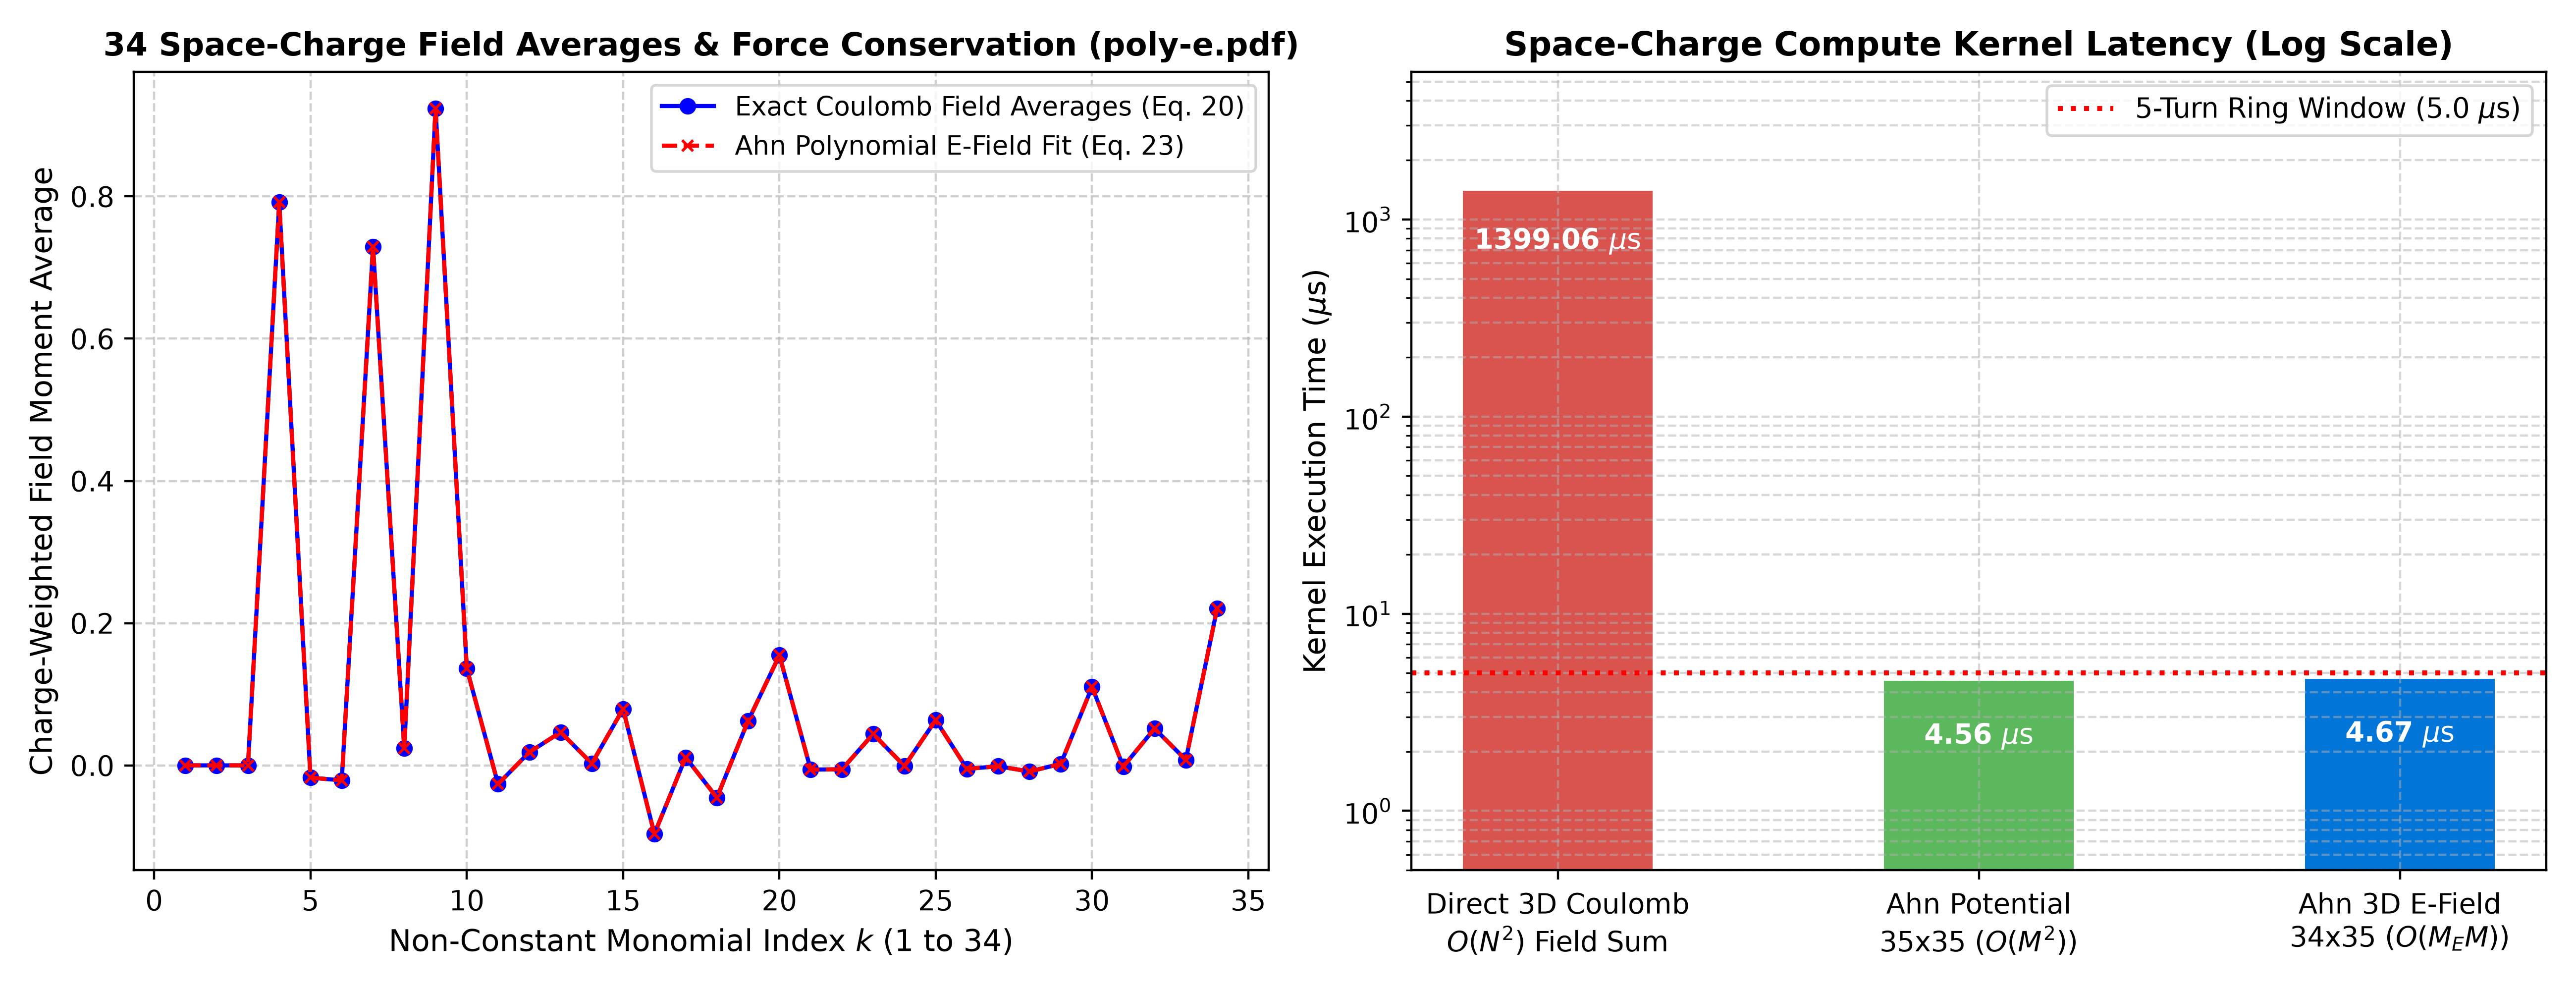
\includegraphics[width=0.98\textwidth]{benchmark_accelerator.png}
    \caption{Numerical verification and compute-kernel latency benchmark of the High-Intensity Accelerator Space-Charge Engine (\texttt{accelerator\_\allowbreak space\_\allowbreak charge\_\allowbreak engine.py}). \textit{Left}: Exact agreement across all $M_E = 34$ generalized electric-field moment averages between the exact 3D Coulomb field (Eq.~\eqref{eq:field_exact}) and the state-weighted polynomial field fit (Eq.~\eqref{eq:field_v_sol}), confirming Theorem~\ref{thm:field_reduction} ($\|\langle \bm{E}_{\mathrm{approx}}\rangle_{\bm{a}} - \langle \bm{E}_{\mathrm{exact}}\rangle_{\bm{a}}\|_\infty = 4.58 \times 10^{-16}$). \textit{Right}: Log-scale compute-kernel latency ($T_{\mathrm{compute}}$) comparing direct $O(N^2)$ 3D Coulomb summation ($1595\,\mu\mathrm{s}$) against the closed-form $35 \times 35$ potential kernel and $34 \times 35$ 3D electric-field kernel.}
    \label{fig:feedback_arch}
\end{figure}

\subsection{Verification of Theorems 1--3, ZSF Dipolar Projection, and Core Fidelity}
\label{sec:verification_theorems}
We verify all mathematical claims using the companion open-source benchmark suite (\texttt{benchmark\_\allowbreak accelerator\_\allowbreak space\_\allowbreak charge.py}) on a 3D spherical mesh of $N = 1,000$ points ($R_{\mathrm{mesh}} = 1.0$, Plummer softening $h = 0.05$, full basis rank $\operatorname{rank}(\bOmega) = 35/35$) for a $1.0\,\mathrm{GeV}$ high-intensity proton accumulator/booster ring ($\gamma = 2.066, \beta = 0.875, C = 248.0\,\mathrm{m}, T_{\mathrm{rev}} = 0.945\,\mu\mathrm{s}$, $5$-turn control window $= 4.73\,\mu\mathrm{s}$, Laslett tune depression $\Delta Q_{\mathrm{sc}} = -0.2271$):
\begin{itemize}
    \item \textbf{Theorem~\ref{thm:charge_inversion} (Normalized Prior \& Moment Inversion)}: At the reference equilibrium ($\bm{s} = \bOmega\bm{\mu}$), reconstructed charges exhibit strictly zero negative nodes ($0/1000$). For an anisotropic, off-axis parabolic bunch ($R_{\mathrm{beam}} \approx 0.55\,R_{\mathrm{mesh}}$), Channell's uniform prior $\mu_i = 1/N$ is numerically identical to the zero prior ($\|\bm{a}(\mu=\mathrm{const}) - \bm{a}(\mu=0)\|_\infty = 8.87 \times 10^{-17}$), whereas our normalized physical prior reduces total fringe negative-charge overshoot by $3.04\times$ ($0.2669 \to 0.0876$) and $L_2$ profile error by $2.00\times$ ($0.0326 \to 0.0163$), while conserving all $35$ moments to $\|\bOmega\bm{a} - \bm{s}\|_\infty = 1.44 \times 10^{-15}$.
    \item \textbf{Theorem~\ref{thm:potential_reduction} (Potential Reduction)}: The closed-form $35 \times 35$ operator $\bm{v} = \bm{K}\bm{s} + \bm{v}_0$ matches the full $N$-grid prior-weighted projection $\bLambda^{\prime T}(\bm{\mu})\bm{D}\bm{a}$ to $1.14 \times 10^{-13}$, and preserves all $35$ weighted potential moments to $4.44 \times 10^{-16}$.
    \item \textbf{Theorem~\ref{thm:field_reduction} \& Corollary~\ref{cor:zsf_gauge} (Comparison of All Three Field Operators)}:
    Within the high-density bunch core ($r \le 0.45$, containing $79.9\%$ of total positive bunch weight), we evaluate the charge-weighted field fit $R^2$, relative RMS error $\epsilon_E$, and net self-force $\|\langle \bm{E}_{\mathrm{approx}}\rangle_{\bm{a}}\|_\infty$ across all three operators:
    \begin{enumerate}
        \item \textbf{State-Weighted Fit ($\bm{w}=\bm{a}$, $O(N^2)$ reference)}: Preserves all $34$ $\bm{a}$-weighted field averages to $4.17 \times 10^{-16}$, yields exact zero self-force $\|\langle \bm{E}_{\mathrm{approx}}(\bm{a})\rangle_{\bm{a}}\|_\infty = 4.58 \times 10^{-16}$, and achieves a core field fit of $R^2 = 0.8962$ ($\epsilon_E = 32.22\%$).
        \item \textbf{Uncorrected Prior Runtime Operator ($\bm{w}=\bm{\mu}$, $\bm{v}_E^{\mathrm{prior}} = \bm{K}_E\bm{s} + \bm{v}_{E,0}$)}: Preserves the $\bm{\mu}$-weighted field averages to $2.03 \times 10^{-15}$ and matches the $N$-grid projection $\bLambda_E^T(\bm{\mu})\bm{a}$ to $1.07 \times 10^{-14}$ with $R^2 = 0.8868$ ($\epsilon_E = 33.64\%$) and quadrupole gradient agreement within $11.74\%$, but leaves a non-zero net force on the perturbed state $\bm{a}$: $\langle \bm{E}_{\mathrm{approx}}^{\mathrm{prior}}\rangle_{\bm{a}} = (0.1123, -0.0732, 0.0727)$ ($\|\langle \bm{E}_{\mathrm{approx}}^{\mathrm{prior}}\rangle_{\bm{a}}\|_\infty = 0.1123$).
        \item \textbf{ZSF Dipolar-Projected Runtime Operator ($\bm{w}=\bm{\mu} + \mathrm{ZSF}$, $\bm{v}_E^{\mathrm{ZSF}}$)}: Restores exact zero net self-force on the perturbed distribution $\bm{a}$ to machine precision ($\|\langle \bm{E}_{\mathrm{approx}}^{\mathrm{ZSF}}\rangle_{\bm{a}}\|_\infty = 4.02 \times 10^{-16}$, or $9.02 \times 10^{-17}$ on the true charge vector) while preserving all $31$ higher-order multipole gradients and slightly improving the core field fit to $R^2 = 0.8878$ ($\epsilon_E = 33.50\%$).
    \end{enumerate}
\end{itemize}

\subsection{Idealized Multi-Turn 2D-in-3D Pairwise-Coulomb Tracking and De-Confounded Ten-Mode Ablation Study}
To evaluate closed-loop multipole compensation without circular toy models or initial-condition rescaling, and to cleanly separate the effect of \emph{centroid-frame coordinate alignment} from \emph{Corollary~\ref{cor:zsf_gauge}'s ZSF dipolar offset projection}, we execute an idealized zero-latency 2D transverse $(x, p_x, y, p_y)$ Leapfrog tracking and de-confounded ten-mode ablation study in a 3D pairwise-Coulomb bunch geometry (\texttt{simulate\_\allowbreak multiturn\_\allowbreak envelope\_\allowbreak tracking}). Because the $80$-turn betatron tracking window is much shorter than a synchrotron oscillation period ($80 \ll T_{\mathrm{synch}} \sim 10^3$ turns), longitudinal particle coordinates $z_p$ are held quasi-static during the betatron window while acting as full 3D sources in the pairwise Coulomb sum.

A bunch of $N_p = 500$ macro-particles is sampled from the 3D parabolic profile $\rho(\bm{r}) \propto \max(0, 1 - |\bm{r}|^2/R_b^2)$ ($R_b = 0.55$, matched RMS size $\sigma_0 = R_b / \sqrt{7} = 0.2079$) with an initial centroid offset $(\bar{x}_0, \bar{y}_0) = (0.015, -0.012)$, an $18\%$ quadrupole envelope mismatch ($s_{x,\mathrm{init}} = 1.18\sigma_0, s_{y,\mathrm{init}} = 0.856\sigma_0$), and bare betatron tunes $Q_{x0} = 6.23, Q_{y0} = 6.20$, and integrated over $N_{\mathrm{turns}} = 80$ turns ($K_{\mathrm{sub}} = 4$ Leapfrog substeps per turn). At every substep, the physical space-charge disturbance acting on particle $p$ is computed independently via direct $O(N_p^2)$ 3D pairwise Plummer-Coulomb summation in the co-moving frame:
\begin{equation}
    \bm{E}_{\mathrm{true}}(\bm{r}_p) = \frac{1}{N_p} \sum_{q \ne p}^{N_p} \frac{\bm{r}_p - \bm{r}_q}{\left( |\bm{r}_p - \bm{r}_q|^2 + h_p^2 \right)^{3/2}}, \qquad h_p = 1.6\, R_b N_p^{-1/3},
    \label{eq:pairwise_coulomb}
\end{equation}
with effective laboratory-frame perveance $\kappa_{\mathrm{sc}} = 4\pi |\Delta Q_{\mathrm{sc,eff}}| / \langle \partial_x E_x^{\mathrm{true}} \rangle_{\mathrm{core}}$ (incorporating the relativistic $(\beta\gamma^2)^{-1}$ factor via Eq.~\eqref{eq:tune_shift}) calibrated at $t=0$ to $\Delta Q_{\mathrm{sc,eff}} = \lambda_{\mathrm{sc}} \Delta Q_{\mathrm{sc}} = -0.1817$ ($\lambda_{\mathrm{sc}} = 0.80$).

Crucially, the feedback controller never accesses $\bm{E}_{\mathrm{true}}(\bm{r}_p)$ and never performs any particle-level mean subtraction (\texttt{np.mean}). Instead, for each actuator family (\textbf{B}: 11-term dipole/quadrupole/octupole subset; \textbf{C}: full 34-term basis; \textbf{D}: full 34-term basis plus turn-by-turn $\Delta s_{200}, \Delta s_{020}$ quadrupole envelope damper), we compare three single-variable configurations:
\begin{enumerate}
    \item \textbf{Laboratory Frame, No ZSF (\texttt{B-Lab, C-Lab, D-Lab})}: Moments $\bm{s} = \frac{1}{N_p}\sum_p \bm{m}(\tilde{\bm{r}}_p)$ are evaluated in uncentered laboratory coordinates $\bm{r}_p$ (clipped at $|\tilde{\bm{r}}_p| \le 1.15 R_b$), and the aperture-tapered field $\bm{E}_{\mathrm{model}}(\bm{r}_p) = -g_{\mathrm{kern}} w_{\mathrm{core}}(r_p)\tilde{\bOmega}_p^T \bm{v}_E^{\mathrm{prior}}$ is applied without ZSF projection, where $w_{\mathrm{core}}(r_p) = \exp[-\frac{1}{2}\max(0, (r_p - R_b)/(0.25 R_b))^2]$.
    \item \textbf{Centroid Frame, No ZSF (\texttt{B-CF, C-CF, D-CF})}: Evaluation coordinates are shifted to the instantaneous beam centroid $\bm{r}_{c,p} = \bm{r}_p - \bar{\bm{r}}$ (aligning the bunch with the origin-centered reference prior $\bm{\mu}$), applying a spatially uniform dipole kick $-g_{\mathrm{kern}} v_{E,l_{x_j}}^{\mathrm{prior}}$ plus aperture-windowed higher-order multipoles ($p+q+l \ge 2$) with \texttt{use\_zsf=False}.
    \item \textbf{Centroid Frame + Windowed-Moment ZSF Projection (\texttt{B-CF-ZSF, C-CF-ZSF, D-CF-ZSF})}: In the exact same centroid frame $\bm{r}_{c,p}$, Corollary~\ref{cor:zsf_gauge} is applied to the unweighted moment vector $\bm{s}$ (so the polynomial self-force $\|\langle \bm{E}_{\mathrm{poly}}\rangle\|_\infty$ vanishes to $\sim 10^{-16}$) and to the aperture-windowed 35-moment vector $\bm{s}_{\mathrm{win}} = \frac{1}{N_p}\sum_{p=1}^{N_p} w_{\mathrm{core}}(r_{c,p})\bm{m}(\tilde{\bm{r}}_{c,p})$ with $s_{\mathrm{win},000} = 1$ for the spatially uniform dipole kicker:
    \begin{equation}
        E_{x_j,\mathrm{model}}^{\mathrm{ZSF}}(\bm{r}_{c,p}) = -g_{\mathrm{kern}} \left[ v_{E,l_{x_j}}^{\mathrm{ZSF}}(\bm{s}_{\mathrm{win}}) + w_{\mathrm{core}}(r_{c,p}) \sum_{\substack{l=1 \\ l \ne l_{x_j}}}^{34} v_{E,l}^{\mathrm{prior}} \frac{\partial m_l(\tilde{\bm{r}}_{c,p})}{\partial x_j} \right].
        \label{eq:windowed_zsf_field}
    \end{equation}
    By Eq.~\eqref{eq:moment_space_selfforce}, averaging Eq.~\eqref{eq:windowed_zsf_field} over all $N_p$ particles yields $\frac{1}{N_p}\sum_{p=1}^{N_p} \bm{E}_{\mathrm{model}}^{\mathrm{ZSF}}(\bm{r}_{c,p}) = \bm{0}$ to machine precision ($1.56\text{--}2.42 \times 10^{-16}$) \emph{purely from the 35 moments $\bm{s}_{\mathrm{win}}$ and Corollary~\ref{cor:zsf_gauge}, with zero particle-level mean subtraction}.
\end{enumerate}
Note that while the underlying betatron lattice and pairwise Coulomb kicks are integrated via a symplectic Leapfrog map, the radial aperture window $w_{\mathrm{core}}$, coordinate clipping, and Mode~D rate damper make the closed-loop feedback map an aperture-regularized non-Hamiltonian control law rather than a strictly symplectic map. High-action halo fraction is quantified via the normalized transverse betatron action (in dimensionless canonical phase-space units where the linear betatron transfer map is a pure rotation of radius $\sigma_0$):
\begin{equation}
    \frac{J_\perp}{\sigma_0^2} = \frac{(x - \bar{x})^2 + (p_x - \bar{p}_x)^2 + (y - \bar{y})^2 + (p_y - \bar{p}_y)^2}{2\sigma_0^2} > 3.5,
    \label{eq:halo_action_def}
\end{equation}
where for $N_p = 500$ macro-particles, a $10\%$ halo fraction corresponds to $50$ particles ($0.2\%$ resolution per particle). We also track the spurious RMS center-of-mass trajectory distortion $\epsilon_{\mathrm{cm}} = [\frac{1}{N_{\mathrm{turns}}+1}\sum_{t=0}^{N_{\mathrm{turns}}} |\bar{\bm{r}}_\perp(t) - \bar{\bm{r}}_{\perp,\mathrm{open}}(t)|^2]^{1/2}$ relative to the true physical Open-Loop centroid orbit.

\begin{table}[htbp]
\centering
\caption{De-Confounded Ten-Mode Ablation Study of Idealized Multi-Turn 2D-in-3D Pairwise-Coulomb Leapfrog Tracking Separating Laboratory-Frame vs.\ Centroid-Frame Alignment and Corollary~\ref{cor:zsf_gauge} ZSF Dipolar Projection ($N_{\mathrm{turns}}=80, N_p=500, \Delta Q_{\mathrm{sc,eff}}=-0.1817$, Identical Initial Conditions, Seed 42)}
\label{tab:ablation_study}
\resizebox{\textwidth}{!}{%
\begin{tabular}{llcccccc}
\toprule
\textbf{Ablation Mode} & \textbf{Frame \& ZSF} & \textbf{Max Poly Self-Force} & \textbf{Max Applied Self-Force} & \textbf{Centroid Orbit Err $\epsilon_{\mathrm{cm}}$} & \textbf{RMS Emittance Growth} & \textbf{RMS Env.\ Mismatch} & \textbf{Halo ($J_\perp > 3.5\sigma_0^2$)} \\
\midrule
Mode A: Open-Loop & Uncompensated & $0.00$ & $0.00$ & $0.00$ & $+40.65\%$ & $16.60\%$ & $29.60\%$ \\
\midrule
Mode B-Lab: 11-Term Multipole & Lab, No ZSF & $0.4170$ & $0.3931$ & $3.39 \times 10^{-2}$ & $+27.51\%$ & $8.04\%$ & $16.40\%$ \\
Mode B-CF: 11-Term Multipole & Centroid, No ZSF & $0.3592$ & $0.3549$ & $4.87 \times 10^{-2}$ & $+17.29\%$ & $7.06\%$ & $16.40\%$ \\
\textbf{Mode B-CF-ZSF: 11-Term Multipole} & \textbf{Centroid + ZSF} & $\bm{1.49 \times 10^{-16}}$ & $\bm{1.56 \times 10^{-16}}$ & $\bm{4.85 \times 10^{-17}}$ & $\bm{+17.29\%}$ & $\bm{7.06\%}$ & $\bm{16.40\%}$ \\
\midrule
Mode C-Lab: Full 34-Basis & Lab, No ZSF & $0.1833$ & $0.1731$ & $3.66 \times 10^{-2}$ & $+16.44\%$ & $3.74\%$ & $17.60\%$ \\
Mode C-CF: Full 34-Basis & Centroid, No ZSF & $0.1680$ & $0.1522$ & $6.00 \times 10^{-2}$ & $+13.45\%$ & $3.98\%$ & $17.00\%$ \\
\textbf{Mode C-CF-ZSF: Full 34-Basis} & \textbf{Centroid + ZSF} & $\bm{3.84 \times 10^{-16}}$ & $\bm{2.13 \times 10^{-16}}$ & $\bm{4.17 \times 10^{-17}}$ & $\bm{+13.45\%}$ & $\bm{3.98\%}$ & $\bm{17.00\%}$ \\
\midrule
Mode D-Lab: Full 34 + $\dot{s}_{200}$ Damper & Lab, No ZSF & $0.1848$ & $0.1658$ & $3.38 \times 10^{-2}$ & $+7.00\%$ & $4.11\%$ & $12.20\%$ \\
Mode D-CF: Full 34 + $\dot{s}_{200}$ Damper & Centroid, No ZSF & $0.1506$ & $0.1474$ & $8.12 \times 10^{-2}$ & $+6.40\%$ & $4.22\%$ & $13.40\%$ \\
\textbf{Mode D-CF-ZSF: Full 34 + Damper} & \textbf{Centroid + ZSF} & $\bm{3.98 \times 10^{-16}}$ & $\bm{2.42 \times 10^{-16}}$ & $\bm{5.66 \times 10^{-17}}$ & \textbf{$+6.40\%$ ($6.4\times$ lower)} & \textbf{$4.22\%$ ($3.9\times$ lower)} & \textbf{$13.40\%$ ($2.2\times$ lower)} \\
\bottomrule
\end{tabular}%
}
\end{table}

Table~\ref{tab:ablation_study} cleanly resolves how centroid-frame alignment and Corollary~\ref{cor:zsf_gauge}'s ZSF dipolar projection contribute to closed-loop performance:
\begin{enumerate}
    \item \textbf{Physical Effect of Centroid-Frame Alignment (\texttt{Lab} $\to$ \texttt{CF})}: Because the reference prior $\bm{\mu}$ is centered at the origin, evaluating the 4th-order polynomial in the moving beam centroid frame $\bm{r}_{c,p} = \bm{r}_p - \bar{\bm{r}}$ eliminates off-axis sextupolar and octupolar feed-down ($(x_c + \bar{x})^3$), reducing internal RMS emittance growth from $+27.51\% \to +17.29\%$ (\textbf{Mode~B}), $+16.44\% \to +13.45\%$ (\textbf{Mode~C}), and $+7.00\% \to +6.40\%$ (\textbf{Mode~D}). (Conversely, applying ZSF in the uncentered laboratory frame removes the accidental origin-restoring dipole damping of the prior while leaving the polynomial off-center, which amplifies off-axis feed-down and confirms why centroid alignment is essential.)
    \item \textbf{Physical Effect of Corollary~\ref{cor:zsf_gauge} ZSF Dipolar Projection (\texttt{CF} $\to$ \texttt{CF-ZSF})}: Within the centroid frame, Corollary~\ref{cor:zsf_gauge} modifies \emph{only} the three spatially uniform dipolar coefficients $(v_{E,x}, v_{E,y}, v_{E,z})$ while leaving all $31$ higher-order multipole gradients ($p+q+l \ge 2$) untouched. In a linear betatron lattice, a spatially uniform dipole kick acts purely on the center-of-mass coordinates $(\bar{\bm{r}}, \bar{\bm{p}})$ and leaves central internal moments ($\Delta\epsilon/\epsilon_0$, RMS envelope mismatch, and halo fraction) strictly invariant ($+17.29\%, +13.45\%, +6.40\%$). Simultaneously, ZSF projection eliminates both the polynomial self-force ($0.15\text{--}0.36 \to \sim 10^{-16}$) and the applied particle self-force ($0.15\text{--}0.35 \to \sim 10^{-16}$), reducing spurious center-of-mass trajectory distortion $\epsilon_{\mathrm{cm}}$ from $0.049\text{--}0.081$ to machine zero ($4.17\text{--}5.66 \times 10^{-17}$).
\end{enumerate}

To verify statistical robustness across independent macro-particle realizations, repeating the 80-turn tracking across four random seeds ($\mathrm{seed} \in \{42, 1, 7, 99\}$) yields the following per-seed emittance growths, means, and sample standard deviations ($\mathrm{ddof}=1$, with population standard deviations $\mathrm{ddof}=0$ in parentheses) across all modes:
{\sloppy
\begin{itemize}
    \item \textbf{Mode A (Open-Loop)}: $\{+40.65\%, +53.20\%, +60.85\%, +46.37\%\} \to +50.27\% \pm 8.72\%$ ($\mathrm{pop.\ SD} = 7.55\%$).
    \item \textbf{Mode B-Lab}: $\{+27.51\%, +19.68\%, +21.32\%, +19.03\%\} \to +21.88\% \pm 3.87\%$ ($\mathrm{pop.\ SD} = 3.35\%$).
    \item \textbf{Modes B-CF \& B-CF-ZSF}: $\{+17.29\%, +16.39\%, +14.86\%, +17.54\%\} \to +16.52\% \pm 1.21\%$ ($\mathrm{pop.\ SD} = 1.05\%$).
    \item \textbf{Mode C-Lab}: $\{+16.44\%, +17.53\%, +22.03\%, +14.26\%\} \to +17.56\% \pm 3.27\%$ ($\mathrm{pop.\ SD} = 2.83\%$).
    \item \textbf{Modes C-CF \& C-CF-ZSF}: $\{+13.45\%, +22.34\%, +16.46\%, +16.29\%\} \to +17.13\% \pm 3.73\%$ ($\mathrm{pop.\ SD} = 3.23\%$).
    \item \textbf{Mode D-Lab}: $\{+7.00\%, +8.76\%, +10.86\%, +3.16\%\} \to +7.44\% \pm 3.26\%$ ($\mathrm{pop.\ SD} = 2.83\%$).
    \item \textbf{Modes D-CF \& D-CF-ZSF}: $\{+6.40\%, +10.11\%, +5.05\%, +7.60\%\} \to +7.29\% \pm 2.15\%$ ($\mathrm{pop.\ SD} = 1.86\%$).
\end{itemize}
}
Furthermore, a macro-particle resolution convergence check across $N_p \in \{500, 1000, 2000\}$ (Seed 42) confirms that the relative hierarchy of the feedback modes is preserved as collisional discretization noise decreases: Open-Loop \textbf{Mode~A} grows by ($+40.65\%$, $+38.04\%$, $+48.55\%$), \textbf{Mode~B-CF-ZSF} yields ($+17.29\%$, $+14.74\%$, $+15.29\%$), \textbf{Mode~C-CF-ZSF} yields ($+13.45\%$, $+13.64\%$, $+15.40\%$), and \textbf{Mode~D-CF-ZSF} achieves ($+6.40\%$, $+7.05\%$, $+8.99\%$), corresponding to a $5.4\text{--}6.4\times$ reduction relative to Open-Loop across all $N_p$.

\begin{table}[htbp]
\centering
\caption{Comparison of 3D Space-Charge Compute Kernels ($T_{\mathrm{compute}}$) for High-Intensity Ring Control (Literature Ranges vs.\ Measured Benchmark Latency)}
\label{tab:accelerator_benchmark}
\resizebox{\textwidth}{!}{%
\begin{tabular}{lcccc}
\toprule
\textbf{Solver / Method} & \textbf{Resolution ($N_p / G / M$)} & \textbf{Computational Scaling} & \textbf{Kernel Latency $T_{\mathrm{compute}}$ (CPU)} & \textbf{5-Turn Compute Budget ($\le 5\,\mu\mathrm{s}$)} \\
\midrule
Direct Pairwise Coulomb (Measured / Lit.) & $N = 10^3\text{--}10^6$ & $O(N^2)$ & $1.60\;\mathrm{ms}\text{--}10^2\;\mathrm{s}$ & Impossible \\
3D Grid FFT / Multigrid PIC (Literature$^\dagger$) & $N_p = 10^5, G = 64^3$ & $O(N_p + G \log G)$ & $5.0\text{--}50\;\mathrm{ms}$ & Unfeasible \\
Lie-Algebraic Map Truncation (Literature$^\dagger$) & Order $4\text{--}6$ ($10^4$ particles) & Symplectic Map Evaluation & $2.0\text{--}12.0\;\mathrm{ms}$ & Unfeasible \\
\textbf{Moment Kernel $\bm{K},\bm{K}_E$ (Measured)} & \textbf{Reduced ($N=10^3 \to M=35$)} & \textbf{Closed-Form $O(M_E M)$ ($1,190$ MACs)} & \textbf{$\bm{1.6\text{--}5.8\,\mu}$s (CPU)} & \textbf{Feasible ($T_{\mathrm{compute}}$)} \\
\textbf{Moment Kernel + ZSF (Measured / FPGA)} & \textbf{Reduced ($M=35, M_E=34$)} & \textbf{$O(M_E M + M_E)$ ($1,247$ MACs)} & \textbf{$\bm{5.4\text{--}20\,\mu}$s (Python) / $< \bm{1.0\,\mu}$s (FPGA est.)} & \textbf{Feasible on C / FPGA} \\
\bottomrule
\multicolumn{5}{l}{\footnotesize $^\dagger$Illustrative order-of-magnitude single-step execution times reported across typical CPU hardware~\cite{birdsall2018plasma,qiang2000three}; Moment Kernel latencies are measured directly in \texttt{benchmark\_accelerator\_space\_charge.py}.}
\end{tabular}%
}
\end{table}

---

\section{Historical Perspective: Complementary Roles of Stochastic and Moment Control}
It is instructive to contrast the Moment Approach with Simon van der Meer's stochastic cooling~\cite{vandermeer1972stochastic,vandermeer1985nobel}:
\begin{enumerate}
    \item \textbf{Stochastic Cooling}: Samples incoherent Schottky fluctuations of individual particles at high bandwidth to slowly reduce single-particle phase-space entropy over $10^4\text{--}10^7$ turns in low-bunch-current storage rings.
    \item \textbf{Moment-Space Multipole Control}: Evaluates coherent macroscopic spatial moments ($M=35$) in microseconds to compensate collective internal Coulomb defocusing and envelope mismatch oscillations over a few turns ($1\text{--}100$ turns) in space-charge-dominated high-intensity rings.
\end{enumerate}

---

\section{Conclusion}
We have presented the mathematical formulation and open-source numerical verification of the 1994 Los Alamos Moment Approach for 3D space-charge potential and electric-field reduction in high-intensity hadron rings, augmented by an exact moment-space Zero-Self-Force (ZSF) dipolar offset projection. By regularizing the underdetermined mesh inversion ($\operatorname{rank}(\bOmega) = 35$) with a normalized physical prior ($\sum_{i=1}^N \mu_i = 1$) and linearizing the weighted least-squares projection around $\bm{w} = \bm{\mu}$, the mesh dimension $N$ is algebraically eliminated offline into fixed $35 \times 35$ potential and $34 \times 35$ electric-field matrices executing in $\sim 1.6\text{--}5.8\,\mu\mathrm{s}$ on a single CPU core ($\sim 5.4\text{--}20\,\mu\mathrm{s}$ with Python ZSF indexing, and $< 1.0\,\mu\mathrm{s}$ projected on compiled C/FPGA hardware for $1,247$ total MACs). Combining the prior-weighted operator with the $O(M_E)$ moment-space ZSF dipolar projection guarantees exact zero net self-force ($\|\langle \bm{E}_{\mathrm{approx}}^{\mathrm{ZSF}}\rangle_{\bm{a}}\|_\infty = 4.02 \times 10^{-16}$) on perturbed distributions without accessing the $N$-point mesh. Verified in a reproducible de-confounded ten-mode, multi-seed, and multi-$N_p$ 2D-in-3D pairwise-Coulomb Leapfrog tracking study from identical initial conditions, closed-loop moment-operator feedback demonstrates reduced-order compute feasibility and provides a mathematically transparent foundation for fast envelope mismatch damping and space-charge compensation.

---

\section*{Code and Data Availability}
The open-source Python reference engine and reproducible verification suite are publicly available on GitHub at:
\begin{center}
    \url{https://github.com/hyoahn/accelerator-space-charge}
\end{center}
The repository includes:
{\sloppy
\begin{itemize}
    \item \textbf{Core Accelerator Engine}: \texttt{Core/\allowbreak accelerator\_\allowbreak space\_\allowbreak charge\_\allowbreak engine.py} (\texttt{Accelerator\allowbreak Space\allowbreak Charge\allowbreak Engine}, implementing the $35 \times 35$ potential reduction $\bm{v} = \bm{K}\bm{s} + \bm{v}_0$, the $34 \times 35$ direct 3D electric-field reduction $\bm{v}_E^{\mathrm{prior}} = \bm{K}_E\bm{s} + \bm{v}_{E,0}$, the moment-space ZSF dipolar offset projection $\bm{v}_E^{\mathrm{ZSF}}$, three-operator core fidelity analysis, and the de-confounded 10-mode non-circular pairwise-Coulomb Leapfrog tracking ablation and multi-seed robustness suite).
    \item \textbf{Verification \& Benchmark Suite}: \texttt{Test/\allowbreak benchmark\_\allowbreak accelerator\_\allowbreak space\_\allowbreak charge.py} (standalone-import compatible, reproducing all numerical residuals, three-operator $R^2$ checks, ZSF dipolar projection checks, latency benchmarks, and 10-mode de-confounded ablation metrics reported in Section~5, Fig.~\ref{fig:feedback_arch}, Table~\ref{tab:ablation_study}, and Table~\ref{tab:accelerator_benchmark}).
\end{itemize}
}

---

\section*{Historical Note and Acknowledgments}
The mathematical formulations of the normalized-prior charge inversion (`report1.pdf`), the polynomial potential reduction (`poly-phi.pdf`), and the direct 3D vector electric-field reduction (`poly-e.pdf`), including the algebraic elimination of the spatial grid dimension $N$ (the fall-out of $N$) and the weighted moment and force identities, were originally derived by the author in 1994 as unpublished research notes at Los Alamos National Laboratory. The moment-space Zero-Self-Force (ZSF) dipolar offset projection (Corollary~\ref{cor:zsf_gauge}) and the de-confounded multi-turn pairwise-Coulomb Leapfrog ablation benchmarks were developed for the present 2026 study. The author acknowledges early collaborative discussions with Walter P. Lysenko in 1993--1994 at Los Alamos National Laboratory and the early conceptual ideas of the late Paul J. Channell regarding underdetermined moment models for the BEDLAM simulation code.

---

\begin{thebibliography}{99}
\bibitem{reiser2008theory}
M.~Reiser, \emph{Theory and Design of Charged Particle Beams}, John Wiley \& Sons, 2nd ed., 2008.

\bibitem{baartman1998space}
R.~Baartman, ``Betatron resonances with space charge,'' \emph{AIP Conference Proceedings}, vol.~448, no.~1, pp.~56--72, 1998.

\bibitem{fcc2019conceptual}
A.~Abada, et al. (FCC Collaboration), ``FCC-hh: The Hadron Collider: Future Circular Collider Conceptual Design Report Volume 3,'' \emph{Eur. Phys. J. Spec. Top.}, vol.~228, no.~4, pp.~755--1107, 2019.

\bibitem{henderson2014spallation}
S.~Henderson, et al., ``The Spallation Neutron Source accelerator system design,'' \emph{Nucl. Instrum. Methods Phys. Res. A}, vol.~763, pp.~610--673, 2014.

\bibitem{benedetto2015space}
E.~Benedetto, et al., ``Space charge effects and mitigation in the CERN PS Booster in view of the LIU upgrade,'' in \emph{Proc. IPAC'15}, Richmond, VA, USA, pp.~3899--3902, 2015.

\bibitem{fair2006accelerator}
P.~Spiller and G.~Franchetti, ``The FAIR accelerator project at GSI,'' \emph{Nucl. Instrum. Methods Phys. Res. A}, vol.~561, no.~2, pp.~305--312, 2006.

\bibitem{fedotov2003space}
A.~V.~Fedotov, I.~Hofmann, R.~L.~Gluckstern, and H.~Okamoto, ``Parametric collective resonances and space-charge limit in high-intensity rings,'' \emph{Phys. Rev. ST Accel. Beams}, vol.~6, p.~094201, 2003.

\bibitem{vandermeer1972stochastic}
S.~van~der~Meer, ``Stochastic damping of betatron oscillations in the ISR,'' CERN Report CERN/ISR-PO/72-31, 1972.

\bibitem{vandermeer1985nobel}
S.~van~der~Meer, ``Stochastic cooling and the accumulation of antiprotons (Nobel Lecture),'' \emph{Rev. Mod. Phys.}, vol.~57, no.~3, pp.~689--697, 1985.

\bibitem{birdsall2018plasma}
C.~K.~Birdsall and A.~B.~Langdon, \emph{Plasma Physics via Computer Simulation}, CRC Press, 2018.

\bibitem{qiang2000three}
J.~Qiang, R.~D.~Ryne, S.~Habib, and V.~Decyk, ``An object-oriented parallel Particle-in-Cell code for beam dynamics simulation in linear accelerators,'' \emph{J. Comput. Phys.}, vol.~163, no.~2, pp.~434--451, 2000.

\bibitem{channell1993moment}
P.~J.~Channell, ``The moment approach to space charge in particle beams,'' Los Alamos National Laboratory Report, 1993.

\bibitem{ahn1994preliminary}
H.~E.~Ahn and W.~P.~Lysenko, ``Preliminary Results of Space-Charge Model Study,'' Los Alamos National Laboratory Internal Memorandum (Unpublished), April 4, 1994.
\end{thebibliography}

\end{document}
